% !TEX root = main.tex

\chapter{Background}
\label{ch:background}
\noindent

\red{TODO: fix fig name}


\section{WebAssembly}
\label{sec:webassembly}


% breif overview
WebAssembly~\cite{wasm} is a low-level bytecode language that is safe, fast,
portable, and compact.
It is widely used as a compile target for web applications.
Not only that, other areas such as edge computing~\cite{wasm-edge},
IoT~\cite{wasm-iot}, and block chains~\cite{wasm-block} deploy the advantages
of WebAssembly.


% risk of implementation divergence
There are dozens of WebAssembly engines; all the browsers have there own
implementations of WebAssembly with multiple tiers ~\cite{v8}
\cite{spidermonkey} \cite{webkit}, and there are many engines that target for
specific areas including embedded systems and edge computing.
However, as WebAssembly should be portable across these implementations, it risks
the implementations divergence.


% rigorous standardization -> spec is rigorous: formal notation & prose notation
To mitigate this problem, WebAssembly has been standardized very rigourously by
the W3C~\cite{wasm-w3c}.
Especially, WebAssembly specification document is written very rigorously.
It describes the semantics of WebAssembly in two forms: formal notation and
prose notation.
Formal notation uses mathematical rules to compactly describe the semantics,
and it is used for proofs such as type soundness.
On the other hand, prose notation uses psudocodes algorithm to explain the
semantics through a step by step instruction.
Most WebAssembly users and engine developers are not familiar with
mathematical rules, so they utilize the prose notation.


% structure
A WebAssembly program is comprised of \textit{modules}.
A module is the unit of deployment, loading, and compilation, which consists of
definitions such as functions, globals, and memories.
A module is instantiated to validate the module and allocate each definition to
the data structure named \textit{store}.
This results in a module instance, a runtime representation for the module.
After the instantiation, functions can be invoked so that the function body,
which is a sequence of instructions, is executed.

\begin{figure}[t]
    \centerline{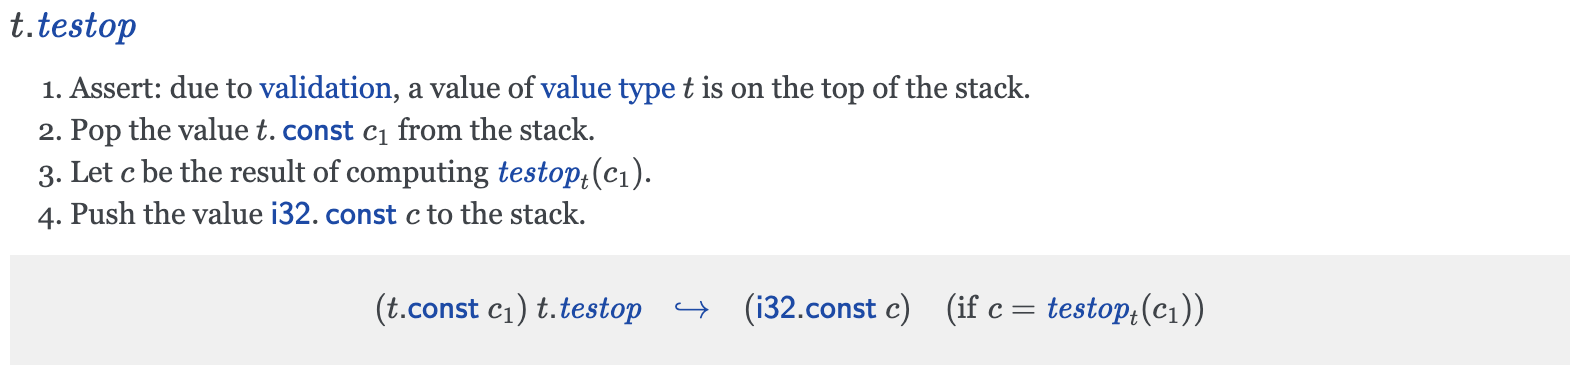
\includegraphics[width=15cm]{fig/testop}}
    \caption[Enter the caption title here]{\texttt{testop} instruction} \label{fig:testop}
    \centerline{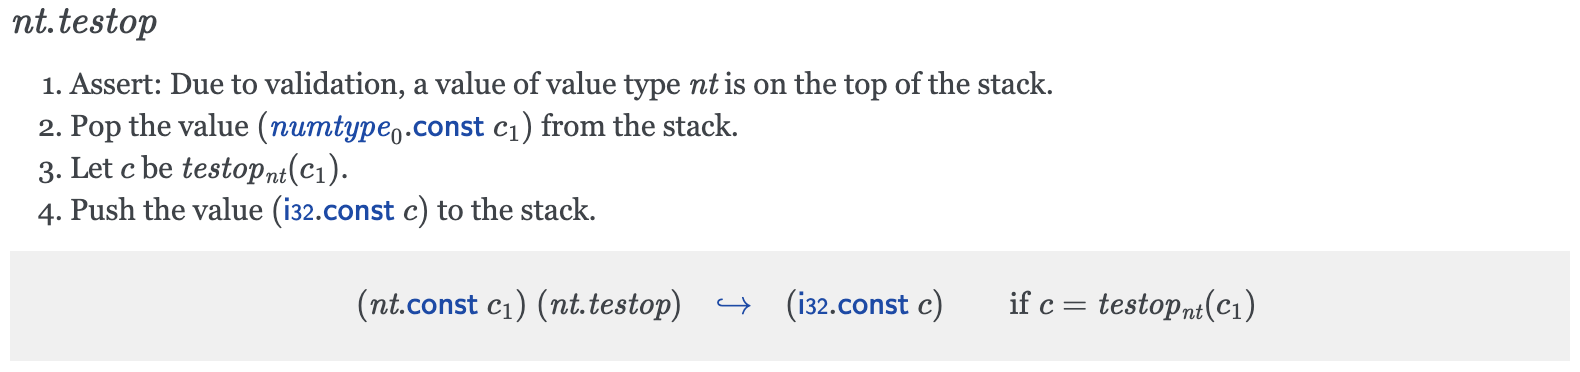
\includegraphics[width=15cm]{fig/spectec-testop}}
    \caption[Enter the caption title here]{SpecTec \texttt{testop} instruction} \label{fig:spectec-testop}
\end{figure}


% execution
WebAssembly execution is based on a stack machine.
An instruction consumes values in the stack as operands, performs some
operation, produces resulting values, and pushes them to the stack.
\cref{fig:testop} is the WebAssembly specification document for the
\texttt{testop} instruction.
Prose notation is written in the upper part, and formal notation is written in
the lower grey box.
In the prose notation, it pops a value from the stack, performs a test
operation, and pushes the result to the stack.
It is written compactly in the form of reduction rule in the formal notation
which consists of LHS, RHS, and premises: $(t.const ~ c_1) ~ t.testop$,
$(i32.const ~ c)$, and $c = testop_t(c_1)$.
The LHS means that the value at the top of the stack is $(t.const ~ c_1)$,
and an instruction to execute is $t.testop$.
The RHS means that the value at the top of the stack is changed to $(i32.const
~ c)$, and this happens when the premise $c = testop_t(c_1)$ is satisfied.


% control structure
The stack stores not only the input and output values of the instructions but also
structures related to the control flow.
A \textit{call frame} and a \textit{label} are used for function call and
branching, respectively.
In exception handling proposal, there is a \textit{handler} for exception
handling, and other strucutres could be introduced in the future.
How these control structures are used for the control flow will be discussed in
\cref{sec:control flow in official prose}.



\section{SpecTec}
\label{sec:spectec}


% SpecTec: specification mechanization tool
SpecTec is a tool for \textit{mechanizing} WebAssembly specification
~\cite{spectec}.
Specification mechanization is a technique that treats a specification as data
that can be manipulated by a computer to automatically generate parser and
interpreter ~\cite{jiset}, to generate tests and perform differential tests
~\cite{jest}, to find meta-level errors in the specification ~\cite{jstar}, and
to perform meta-level static analysis for the static analysis of the defined
language ~\cite{jsaver}.
This technique is especially crucial in growing languages such as JavaScript
and WebAssembly.


% DSL high-level explanation
SpecTec provides a domain specific language (DSL) for the specification.
The DSL is a declarative language that resembles textbook style notation.
It is type checked to prevent meta-level errors such as notation misuses and
dimension mismatches. The code below is the specification for \texttt{testop}
instruction written in the DSL, which is designed to be similar to the formal
notation when describing the semantics with compact and user-friendly
notation.
\\
\red{TODO: better character for $\sim$ in the code}
\begin{verbatim}
  rule Step_pure/testop:
  (CONST nt c_1) (TESTOP nt testop)  ~>  (CONST I32 c)
  -- if c = $testop_(nt, testop, c_1)
\end{verbatim}


% DSL
The DSL consists of DSL definitions.
There are mainly 4 kinds of DSL definitions: type, grammar, relation, and
functions.
Type definitions are used to define abstract syntax, while grammar definitions
are used to define concrete syntax.
Relation definitions are used to define semantics; the code above is also
described in relation definition.
Function definitions can be utilized for other definitions such as
\texttt{\$testop\_} in the code.
In addition, they can be also used to describe semantics.
Especially, SpecTec uses function definitions to describe module instantiation
and function invocation.


% AL
However, The DSL cannot generate the prose notation just as it is because it is
declarative.
Therefore, SpecTec also defines another imperative language \textit{AL}, which
stands for algorithmic language, for the prose notation.
SpecTec translates the semantics describing part of the DSL, which is the
relation defintions and the function definitions, into the AL.
Both definitions are expressed in the form of algorithms in AL that takes some
inputs and performs a step by step instructions as in the prose notation.


% meta-level interpreter
What is especially intriguing here is that AL is executable.
It can perform each step written in the prose program one by one, which
WebAssembly interpreter should follow.
As a result, the prose program serves as a WebAssembly interpter.
That is to say, if WebAssembly semantics is written in the DSL, SpecTec
automatically generates the WebAssembly interpreter following the written
semantics.
The generated interpreter passes all the execution tests in the official test
suites except for the tests related to the infinte loop.


% artifacts SpecTec generates & SpecTec for other language
\cref{fig:spectec-testop} is the specification document generated by the
SpecTec using the DSL and the AL.
The generated document closely resembles the official document except for some
minor notation changes and some missing hyperlinks.
Additionally, SpecTec can generate many other artifacts automatically from the
DSL.
SpecTec translates the DSL into Coq for mathematical proofs and is working
on generating other artifacts, such as test suites required for WebAssembly
standardization.
Furthermore, research is ongoing to extend SpecTec for mechanizing other
languages ~\cite{p4-cherry-workshop}.
